\documentclass[final]{header/fhnwreport}

\input{header/header}

\makeatletter
\newcommand{\vect}{\mathpalette{\overarrowsmall@\rightharpoonfill@}}
\def\rightharpoonfill@{\arrowfill@\relbar\relbar\rightharpoonup}
\newcommand{\overarrowsmall@}[3]{
	\vbox{
		\ialign{
			##\crcr
			#1{\smaller@style{#2}}\crcr
			\noalign{\nointerlineskip}
			$\m@th\hfil#2#3\hfil$\crcr
		}
	}
}
\def\smaller@style#1{
	\ifx#1\displaystyle\scriptstyle\else
	\ifx#1\textstyle\scriptstyle\else
	\scriptscriptstyle
	\fi
	\fi
}
\makeatother

\newenvironment{conditions}
{\par\vspace{\abovedisplayskip}\noindent\begin{tabular}{>{$}l<{$} @{${}={}$} l}}
	{\end{tabular}\par\vspace{\belowdisplayskip}}

\title{\textbf{{\Huge E 6 - Magnetic Fields}}}
\author{{\Huge Physics Laboratory Report}}
\date{{\LARGE Windisch, \the\day.\MONTH \the\year}}

\begin{document}

% Physics Laboratory Notebook
\pagenumbering{gobble}
\selectlanguage{english}
\newpage
\null
\setlength{\unitlength}{1cm}
\begin{picture}(0,0)
	\linethickness{0.025mm}
	\put(-0.85,2.2){\mbox{\includegraphics[height=12mm]{fhnw-logo/fhnw_ht_logo_en}}}
\end{picture}
\par
\textbf{\Huge Physics Laboratory Notebook}
\vskip 1cm
\begin{LARGE}
	\setlength\tabcolsep{0pt}
	\begin{tabularx}{\textwidth}{l p{0.9cm} X}
		\textbf{Experiment Leader:} & & Dominik Müller \\
		\textbf{Assistant:} & & Nico Canzani \\
	\end{tabularx}
\end{LARGE}
\vskip 1.5cm
\begin{center}
	\begin{Large}
		\begin{tabularx}{\textwidth}{l|X|l|l}
			\textbf{Date} & \textbf{Experiment} & \textbf{Due Date} & \textbf{Accepted} \\
			\hline\hline
			& & & \\
			12.03.2019 & W 12 - Ultrasound & 24.05.2019 & \\
			& & & \\
			\hline
			& & & \\
			09.04.2019 & A 8 - Light Quantum & 07.06.2019 & \\
			& & & \\
			\hline
		\end{tabularx}
	\end{Large}
\end{center}
\clearpage


% Title
\selectlanguage{English}
\maketitle
\vfill
\begin{LARGE}
	\begin{tabularx}{\textwidth}{l p{0cm} X}
		\hline
		& & \\
		\textbf{Experiment Leader:} & & Dominik Müller \\
		\textbf{Assistant:} & & Simon Burkhardt \\
	\end{tabularx}
\end{LARGE}
\clearpage

% Contents
\pagenumbering{Roman}		
\selectlanguage{English}
\tableofcontents
\clearpage

% Text
\pagenumbering{arabic}
\selectlanguage{English}
\section{Theoretical Foundations}
\label{sec:Theoretical_Foundations}
This section summarizes the theory and formulas necessary to understand the following experiments on the magnetic field in section \ref{sec:Evaluation}.

\subsection{Magnetic Flux Density}
\label{subsec:Magnetic_Flux_Density}
The decisive factor for the magnetic interactions is the magnetic flux density $\vect{B}$. In a vacuum or in the air, it is proportional to the magnetic field strength $\vect{H}$ \cite{magnetic_fields}.

The magnetic field strength $\vect{H}$ is used to calculate the magnetic flux density $\vect{B}$:
\begin{equation}
\vect{B}=\mu_0 \cdot \mu_r \cdot \vect{H} \qquad \text{with} \qquad
\begin{cases} 
	\mu_0=4\pi\cdot 10^{-7}\ \,^\text{Vs}\!/_\text{Am}\\
	\mu_r=1 \qquad \text{for vacuum or air} \\
\end{cases}
\label{eq:magnetic_flux_density}
\end{equation}
where:
\begin{conditions}
	\vect{B} & magnetic flux density \\
	\vect{H} & magnetic field strength \\
	\mu_0 & vacuum permeability \\
	\mu_r & relative permeability
\end{conditions}

\subsection{Calculating Magnetic Fields}
\label{subsec:Calculating_Magnetic_Fields}
The relationship between the electric current and the magnetic field generated by it can be formulated in two different ways. Either in an integral form with the Ampère's circuital law or in a differential form with the Biot-Savart law \cite{magnetic_fields}.
\addtocontents{toc}{\protect\setcounter{tocdepth}{2}}
\subsubsection{Ampère's circuital law}
\addtocontents{toc}{\protect\setcounter{tocdepth}{3}}
\label{subsubsec:Amperes_circuital_law}
Ampère's circuital law describes the total current $\Theta$ that passes through the area $A$, which is enclosed by the curve $\Gamma$ (graphically shown in figure \ref{fig:amperes_circuit_law}). The following formula is only suitable for the calculation of a symmetrical magnetic field, even though it is valid in any situation \cite{magnetic_fields}.
\begin{equation}
\Theta=\oint_\Gamma \,^{\vect{B}}\!/_{\mu} \cdot\vect{\text{d}l}=\oint_\Gamma \vect{H}\cdot\vect{\text{d}l}=\int \vect{j}\cdot \vect{\text{d}A}
\end{equation}
where:
\begin{conditions}
	\vect{B} & magnetic flux density \\
	\vect{H} & magnetic field strength \\
	\mu & permeability of a specific medium \\
	\vect{\text{d}l} & infinitesimal element of the curve $\Gamma$ \\
	\vect{j} & current density \\
	\vect{\text{d}A} & vector area of an infinitesimal element of the area A
\end{conditions}
\begin{figure}[H]
	\centering
	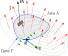
\includegraphics[scale=1]{amperes_circuit_law}
	\caption{Graphical representation of the Ampère's circuital law \cite{magnetic_fields} - partially modified}
	\label{fig:amperes_circuit_law}
\end{figure}
\addtocontents{toc}{\protect\setcounter{tocdepth}{2}}
\subsubsection{Biot-Savart law}
\addtocontents{toc}{\protect\setcounter{tocdepth}{3}}
\label{subsubsec:Biot-Savart_law}
The Biot-Savart law describes the contribution of a current path to the magnetic field at the point P. The resulting total magnetic field at the point P can be calculated by the integration over the whole conductor (graphically shown in figure \ref{fig:biot-savart_law}). This law can always be applied because it is based on the known geometry of the conductor \cite{magnetic_fields}.
\begin{equation}
\text{d}\vect{B}=\mu\cdot \text{d}\vect{H}=\frac{1}{4\pi|\vect{r}-\vect{r}_\text{L}|^2}\cdot\mu\cdot I\cdot\vect{\text{d}l}\times\frac{(\vect{r}-\vect{r}_\text{L})}{|\vect{r}-\vect{r}_\text{L}|}
\label{eq:biot-savart_law}
\end{equation}
where:
\begin{conditions}
	\vect{B} & magnetic flux density \\
	\vect{H} & magnetic field strength \\
	\mu & permeability of a specific medium \\
	I & current path \\
	\vect{\text{d}l} & infinitesimal element of the current path $I$
\end{conditions}
\begin{figure}[H]
	\centering
	\includegraphics[scale=0.35]{biot-savart_law}
	\caption{Graphical representation of the Biot-Savart law \cite{magnetic_fields}}
	\label{fig:biot-savart_law}
\end{figure}
\newpage
\subsection{Measuring Magnetic Fields}
\label{subsec:Measuring_Magnetic_Fields}
The most common method to measure the magnetic flux density (see equation \ref{eq:magnetic_flux_density}) is to use a Hall effect sensor. A known current flows through a thin rectangular plate of a conductive material (usually a semiconductor). At the same time it is penetrated by the magnetic field $\vect{B}$. This results in an electrical field $\vect{F}_{\text{el.}}$ which is perpendicular to the current and the magnetic field. Furthermore, in equilibrium it compensates the Lorentz force $\vect{F}_L$. This means that the Lorentz force is equal to the electrical field ($\vect{F}_L=\vect{F}_{\text{el.}}$). The so-called Hall voltage can be measured at the narrow sides of the plate \cite{magnetic_fields}.
\begin{equation}
U_H=\frac{1}{N\cdot q\cdot d}\cdot I\cdot B\qquad \text{with}\qquad q=-e=-1.602\cdot 10^{-19}\ \text{C}
\end{equation}
where:
\begin{conditions}
	U_H & Hall voltage \\
	N & charge carrier density \\
	q & elementary charge \\
	d & thickness of the plate \\
	I & current \\
	B & magnetic field
\end{conditions}
Since the conductive material used in Hall sensors is usually a temperature-dependent semiconductor, alternating current (e.g. 1 kHz) is used to compensate thermoelectric voltages \cite{magnetic_fields}.
\begin{figure}[H]
	\centering
	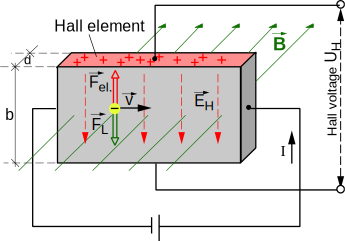
\includegraphics[scale=1]{hall_element}
	\caption{Construction of a Hall element \cite{magnetic_fields} - partially modified}
	\label{fig:hall_element}
\end{figure}

\subsection{Cylindrical Coil}
\label{subsec:Cylindrical_Coil}
For the derivation of the magnetic field of a cylindrical coil, it is assumed that the coil is of length $l$, with a diameter of $2R$ and $N$ turns (one or two layer wound). For the construction see figure \ref{fig:cylindrical_coil}. The following derivation is based on the Biot-Savart law (see equation \ref{eq:biot-savart_law}) \cite{magnetic_fields}.

First, the discrete winding current is replaced by an equivalent surface current $j_{2-d}$:
\[
N\cdot I=l\cdot j_{2-d}
\]
This results in a current segment with the length $\text{dz}_\text{L}$ which represents a cylindrical coil with the radius $R$ and the current:
\[
\text{d}I=j_{2-d}\cdot \text{dz}_\text{L}
\]
Its contribution to the magnetic field at the point P is:
\[
\text{d}B_z=\frac{\mu_0\cdot R^2}{2}\cdot\frac{\text{d}I}{\left[(z-z_\text{L})^2+R^2\right]^{\,^{3}\!/_{2}}}=\frac{\mu_0\cdot N\cdot I \cdot R^2}{2l}\cdot\frac{\text{dz}_L}{\left[(z-z_\text{L})^2+R^2\right]^{\,^{3}\!/_{2}}}
\]
To obtain the magnetic field $B$ at the position $z$, one has to integrated over the entire length of the coil (from $\,^{-l}\!/_{2}$ to $\,^{+l}\!/_{2}$):
\[
B_z(z)=\frac{\mu_0\cdot N\cdot I \cdot R^2}{2l}\cdot\int_{\,^{-l}\!/_{2}}^{\,^{+l}\!/_{2}}\frac{1}{\left[(z-z_\text{L})^2+R^2\right]^{\,^{3}\!/_{2}}}\cdot\text{dz}_L
\]
This results in the following equation for the magnetic field $B_z$:
\begin{equation}
B_z(z)=\frac{\mu_0 N I}{l}\cdot\frac{1}{2} \left[\frac{\,^{l}\!/_{2}+z}{\sqrt{(\,^{l}\!/_{2}+z)^2+R^2}}+\frac{\,^{l}\!/_{2}-z}{\sqrt{(\,^{l}\!/_{2}-z)^2+R^2}}\right]
\label{eq:cylindrical_coil_bz}
\end{equation}
To obtain the magnetic field in the center of the coil $B_z(z=0)$, the following equation is used:
\begin{equation}
B_0=B_z(0)=\frac{\mu_0 N I}{l}\cdot \frac{1}{\sqrt{1+(\,^{2R}\!/_{l})^2}}
\label{eq:cylindrical_coil_b0}
\end{equation}
where:
\begin{conditions}
	B_z & magnetic field at the position z \\
	B_0 & magnetic field in the center \\
	\mu_0 & vacuum permeability \\
	N & number of turns \\
	I & current \\
	l & length \\
	z & position \\
	R & radius
\end{conditions}
\begin{figure}[H]
	\centering
	\includegraphics[scale=0.25]{cylindrical_coil}
	\caption{Construction of a Cylindrical Coil \cite{magnetic_fields}}
	\label{fig:cylindrical_coil}
\end{figure}

\section{Conducting the Experiments}
\label{sec:Conducting_the_Experiments}
This section describes the experimental arrangement with the device list and all the measurement objects. Furthermore, it contains information about the measuring process. All measurements were conducted at 21 \textdegree C room temperature.

% -------------------------------------------------------------------------------------------
\subsection{Measurements}
\label{subsec:Measurements}
In this experiment, the following measurements were conducted (exact descriptions of the tasks can be found in the assignment \cite{light_quantum}):

\begin{enumerate}
	\item Photoelectric effect: Direct measurement
	\item Photoelectric effect: Counter-field method
	\item Light-emitting diode: Threshold voltage $U$ and peak wave length $\lambda$
\end{enumerate}

% -------------------------------------------------------------------------------------------
\subsection{Experimental Arrangement}
\label{subsec:experimental_arrangement}
The experiment was arranged as shown below in figure \ref{fig:experimental_arrangement}:
\begin{figure}[H]
	\centering
	\includegraphics[width=\textwidth]{experimental_arrangement_photoeffect_picture}
	\caption{Annotated picture of the experimental arrangement for measurements no. 1 and 2: The photoelectric effect was measured directly and with the counter-field method. The mercury-vapor lamp was running for at least 10 min before any measurements were conducted.}
	\label{fig:experimental_arrangement}
\end{figure}

\newpage
To measure the voltage $U$ and the peak wave length $\lambda$ an oscilloscope and a spectrometer were used. This is shown in figure \ref{fig:experimental_arrangement_led_picture}:

\begin{figure}[H]
	\centering
	\includegraphics[width=\textwidth]{experimental_arrangement_led_picture}
	\caption{Annotated picture of the experimental arrangement for measurement no. 3: The threshold voltage $U$ and the peak wave length $\lambda$ was measured with an oscilloscope and a spectrometer respectively. The function generator was used to power the LEDs. The oscilloscope was configured in the XY time mode to measure the current in function of the voltage.}
	\label{fig:experimental_arrangement_led_picture}
\end{figure}

The following equipment was used:

\begin{table}[H]
	\centering
	\renewcommand{\arraystretch}{1.2}
	\begin{tabular}{l l l}
		\hline
		\textbf{Device} & \textbf{Designation} & \textbf{Uncertainty} \\
		\hline
		Function Generator & HP 33120A & N/A \\
		Vacuum Phototube & CETRON 1P39 & N/A \\
		Power Supply & Philips SO 140 W & N/A \\
		Oscilloscope & LeCroy WaveRunner 6051A (P-06-103) \cite{oscilloscope} & $\pm0.02$ V \\
		Spectrometer & Ocean Optics HR4000CG-UV-NIR (P-O-064) \cite{spectrometer} & $\pm1$ nm \\
		Electrometer & Keithley 617 (P-E11-059) \cite{electrometer} & $\approx0.05$\ \% \\
		Multimeter & Keithley 2000 Multimeter \cite{multimeter} & $\approx6$\ mV \\
		Lamp & Mercury-Vapor (Hg) & N/A \\ \hline
	\end{tabular}
	\caption{List of the used equipment and measurement devices including the test equipment number in brackets, if available. Furthermore, the uncertainty is stated for all of the measurement devices (not for the regular equipment).}
	\label{tab:equipment}
\end{table}

% -------------------------------------------------------------------------------------------
\newpage
\subsection{Measuring Procedure}
\label{subsec:measuring_procedure}
The following picture illustrate the measuring procedure. Figure \ref{subfig:experimental_arrangement_photoeffect} shows the measurement setup for measurements nr. 1 and 2 in detail. Figure \ref{subfig:experimental_arrangement_led} shows a simplified schematic of the LEDs used in experiment nr. 3.

\begin{figure}[H]
	\subfloat[Measuring procedure of the measurements nr. 1 and 2. Two different filters were used to measure certain wave lengths. \label{subfig:experimental_arrangement_photoeffect}]{
		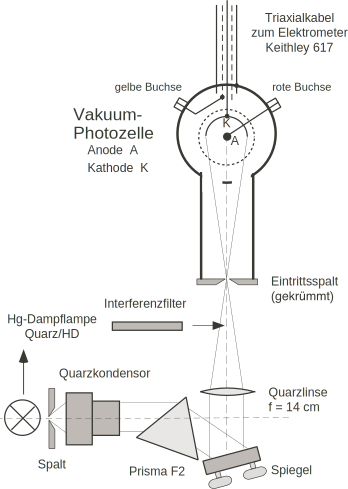
\includegraphics[width=0.45\textwidth]{experimental_arrangement_photoeffect}
	}
	\hfill
	\subfloat[Simplified schematic of the LED connections. A 10 $\Omega$ shunt is used to measure the current. The voltage is measured directly. \label{subfig:experimental_arrangement_led}]{
		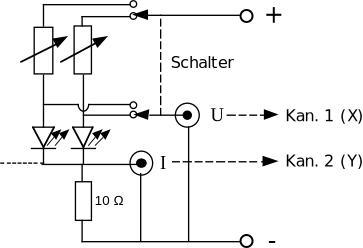
\includegraphics[width=0.45\textwidth]{experimental_arrangement_led}
	}
	\caption{Further diagrams for the conducted experiments. \textbf{(a)} shows the measuring procedure for measurements nr. 1 and 2. \textbf{(b)} shows a simplified schematic of how the LEDs are connected to power and to the oscilloscope in measurement nr. 3.}
	\label{fig:experimental_arrangement_diagram}
\end{figure}


\subsection{Software}
\label{subsec:Software}
All measurements are listed in appendix \ref{sec:Measurements}. The following software was used to record and evaluate the measurements:

\begin{itemize}
	\item Microsoft Office 365 Excel (64-bit)
	\item QtiPlot 0.9.9.2 (64-bit)
	\item Logger Pro 3.8.3 (64-bit)
\end{itemize}

% -------------------------------------------------------------------------------------------
\newpage
\subsection{Measurement Objects}
\label{subsec:measurement_objects}
The measurement objects are a mercury-vapor lamp and several different LEDs.

\paragraph{Mercury-Vapor Lamp}
Figure \ref{fig:hg} shows the spectrum of a mercury-vapor lamp which was measured.

\begin{figure}[H]
	\centering
	\includegraphics[width=\textwidth]{hg}
	\caption{The left picture shows the spectrum of a mercury-vapor lamp. A dispersive prism was used to disperse the light of the lamp. The right picture shows the line spectrum of a mercury-vapor lamp with the most important peaks annotated \cite{mercury-vapor_lamp_picture}. - partially modified}
	\label{fig:hg}
\end{figure}

The photoelectric voltage was measured at the following wave lengths shown in table \ref{tab:hg_colors}:

\begin{table}[H]
	\centering
	\renewcommand{\arraystretch}{1.2}
	\begin{tabular}{cc|c}
		\textbf{Wave length} $\lambda$ \cite{mercury-vapor_lamp} &  & \textbf{Color} \\
		\hline
		\textbf{365.4 nm} &  & Ultraviolet (UVA) \\
		\textbf{404.7 nm} &  & Violet \\
		\textbf{435.8 nm} &  & Blue \\
		\textbf{546.1 nm} & $^{1)}$ & Green \\
		\textbf{578.2 nm} & $^{2)}$ & Orange / Yellow \\ \hline
	\end{tabular}
	\caption{This table lists the wave length and their respective color.}
	\label{tab:hg_colors}
\end{table}

$^{1)}$ To measure the photoelectric voltage at a wavelength of 546.1 nm the filter OG530 was used.
$^{2)}$ To measure the photoelectric voltage at a wavelength of 578.2 nm the filter OG570 was used.

An annotated picture of the used filters can be found in appendix \ref{sec:filters}.

\paragraph{LEDs}
Table \ref{tab:leds} shows the designation of the LEDs that were measured and their respective colors:

\begin{table}[H]
	\centering
	\renewcommand{\arraystretch}{1.2}
	\begin{tabular}{r|l}
		\textbf{Designation} & \textbf{Color} \\
		\hline
		\textbf{L-7113QBC-D} & Blue \\
		\textbf{L-7113SGC} & Green \\
		\textbf{L-7113SYC-H} & Yellow \\
		\textbf{L-7113SEC-H} & Red \\
		\textbf{L-7114QWC-D} & White \\
		\textbf{LD 274} & Infrared \\ \hline
	\end{tabular}
	\caption{This table lists the wave length and their respective color.}
	\label{tab:leds}
\end{table}

\section{Evaluation}
\label{sec:Evaluation}
This section contains the evaluation and the graphical representation of the measurements. The following subsections contain the measurement results of the individual tasks listed in chapter \ref{subsec:Measurements}. The aim is to determine the sound velocity and the attenuation coefficient of different materials. The exact descriptions of the tasks can be found in the assignment \cite{ultrasound}.

%-----------------------------------------------------------------------------------
\subsection{Wave Length Calculation}
\label{subsec:wave_length_calculation}
The following table \ref{tab:wave_length_calculation} shows the calculated wave length $\lambda$ of the ultrasound wave in air, distilled water and aluminium at 1 kHz, 1 MHz and 5 MHz. All literature longitudinal sound velocities are at 20 \textdegree C room temperature.

\begin{table}[H]
	\centering
	\renewcommand{\arraystretch}{1.3}
	\begin{tabular}{r||c|c|c|c}
		& $\boldsymbol{c_L}$ ($\frac{\si{m}}{\si{s}}$) \cite{kohlrausch} & $\boldsymbol{\lambda}$ \textbf{@ 1 kHz} (m) & $\boldsymbol{\lambda}$ \textbf{@ 1 MHz} (m) & $\boldsymbol{\lambda}$ \textbf{@ 5 MHz} (m) \\
		\hline\hline
		\textbf{Air} & 344 & 0.34 & $344\cdot 10^{-6}$ & $68.8\cdot 10^{-6}$ \\
		\textbf{Distilled Water} & 1483 & 1.48 & $1.48\cdot 10^{-3}$ & $297\cdot 10^{-6}$ \\
		\textbf{Aluminium} & 6400 & 6.40 & $6.40\cdot 10^{-3}$ & $1.28\cdot 10^{-3}$ \\
	\end{tabular}
	\caption{Calculated wave lengths $\lambda$ for different solids and liquids at the audible frequency 1 kHz and the two ultrasound frequencies 1 MHz and 5 MHz. The calculations were carried out in the software Microsoft Office Excel.}
	\label{tab:wave_length_calculation}
\end{table}

%-----------------------------------------------------------------------------------
\subsection{Longitudinal Ultrasound Velocities in Solids}
\label{subsec:Longitudinal_Ultrasound_Velocities_in_Solids}
Table \ref{tab:Longitudinal_Ultrasound_Velocities_in_Solids} shows the calculated longitudinal ultrasound velocities from the measurements. These results were obtained using linear regression. This was done in the software QtiPlot. To use linear regression, equation \ref{eq:sound_velocity} has to be rearranged, so that it relates the time of flight with the distance and an offset $b$ has to be added:

\begin{equation}
\Delta t = \frac{2x}{c_L} + b
\label{eq:sound_velocity_linear_regression}
\end{equation}

This equation \ref{eq:sound_velocity_linear_regression} can now be used in QtiPlot.

\begin{table}[H]
	\centering
	\renewcommand{\arraystretch}{1.3}
	\begin{tabular}{r||c|c|c}
		& $\boldsymbol{c_L}$ \textbf{@ 1 MHz} ($\frac{\si{m}}{\si{s}}$) & $\boldsymbol{c_L}$ \textbf{@ 5 MHz} ($\frac{\si{m}}{\si{s}}$) & \textbf{Literature Value} ($\frac{\si{m}}{\si{s}}$) \cite{kohlrausch} \\
		\hline\hline
		\textbf{PMMA} & $(2751\pm 5)$ & $(2721\pm 10)$ & $\approx 2700$ \\
		\textbf{Aluminium} & - & $(6387\pm 30)$ & $\approx 6400$ \\
		\textbf{Copper} & - & $(4680\pm 17)$ & $\approx 4700$ \\
		\textbf{Brass} & - & $(4627\pm 46)$ & $\approx 4700$ \\
	\end{tabular}
	\caption{Measured longitudinal ultrasound velocities $c_L$ in different solids. Furthermore, the literature value of $c_L$ is stated. The literature values are from a physics book from 1968.}
	\label{tab:Longitudinal_Ultrasound_Velocities_in_Solids}
\end{table}

The longitudinal ultrasound velocities of the metals could not be measured with a frequency of 1 MHz. Figure \ref{fig:ghost} shows the measured \flqq ghost signals\frqq\ (signals which are overlapping). Due to this, the longitudinal ultrasound velocities of the metals was only measured with a frequency of 5 MHz, which works perfectly fine.

Figures \ref{fig:Longitudinal_Ultrasound_Velocity_of_PMMA} and \ref{fig:Longitudinal_Ultrasound_Velocity_of_Aluminium} show the plots obtained from QtiPlot for PMMA and aluminium respectively.

\begin{figure}[H]
	\centering
	\includegraphics[scale=0.94]{Longitudinal_Ultrasound_Velocity_of_PMMA}
	\caption{This plot shows the time of flight $\Delta t$ in relation to the distance $x$ for PMMA.Linear regression can then be used on these discrete values to obtain the longitudinal ultrasound velocity of PMMA. The fitted curve is shown in red and the discrete measurements are shown as black dots.}
	\label{fig:Longitudinal_Ultrasound_Velocity_of_PMMA}
\end{figure}

\begin{figure}[H]
	\centering
	\includegraphics[scale=0.94]{Longitudinal_Ultrasound_Velocity_of_Aluminium}
	\caption{Linear regression is used here as well. This time to obtain the longitudinal ultrasound velocity of aluminium. The measurement had to be done at a frequency of 5 MHz because of ghost signals (see figure \ref{fig:ghost}). The fit is shown in red and the measurements as black dots.}
	\label{fig:Longitudinal_Ultrasound_Velocity_of_Aluminium}
\end{figure}

\begin{figure}[H]
	\centering
	\includegraphics[scale=0.5]{ghost}
	\caption{When metals are measured with a transducer that has an oscillation frequency of 1~MHz, \flqq ghost signals\frqq\ occur. This is due to the much higher longitudinal ultrasound velocity of the metals, which leads to signals overlapping also known as \flqq ghost signals\frqq. To get rid of this effect the oscillation frequency can be increased.}
	\label{fig:ghost}
\end{figure}

\newpage
%-----------------------------------------------------------------------------------
\subsection{Attenuation Coefficient of PMMA}
\label{subsec:Attenuation_Coefficient_of_PMMA}
The results for the attenuation coefficient $\mu$ of PMMA are shown in table \ref{tab:Attenuation_Coefficient_of_PMMA} below. The attenuation coefficient $\mu$ was measured with an oscillation frequency of 1 MHz and 5 MHz.

\begin{table}[H]
	\centering
	\renewcommand{\arraystretch}{1.3}
	\begin{tabular}{r||c|c}
		& $\boldsymbol{\mu}$ \textbf{@ 1 MHz} ($m^{-1}$) & $\boldsymbol{\mu}$ \textbf{@ 5 MHz} ($m^{-1}$) \\
		\hline\hline
		\textbf{PMMA} & $(16\pm 1)$ & $(43\pm 3)$ \\
	\end{tabular}
	\caption{Results of the non-linear fit carried out in the software QtiPlot. The unit of the attenuation coefficient $\mu$ has to be m$^{-1}$ due to the fact, that the exponent of $e$ has to be uniform and the distance has the unit m. This leads to the following: $\si{m}^{-1}\cdot \si{m} = 1$.}
	\label{tab:Attenuation_Coefficient_of_PMMA}
\end{table}

To obtain these results, non-linear regression was used. The necessary exponential relationship of the absorption is shown in equation \ref{eq:absorption}. This relationship was used in QtiPlot to create the fit shown in figure \ref{fig:Attenuation_Coefficient_of_PMMA}.

\begin{figure}[H]
	\centering
	\includegraphics[scale=1]{Attenuation_Coefficient_of_PMMA}
	\caption{Semi-log plot of the amplitude $A$ in function of the distance $x$ which shows the attenuation of the signal in PMMA. The black and red line represent the exponential fit of the attenuation. The fits look like a linear function because of the logarithmic y-axis. Furthermore, the attenuation at a lower frequency is less than at a higher frequency, just as expected (see chapter \ref{subsec:Absorption}). Noticeable is the last red measurement value which seems to be off by quite a bit. This is probably due to the small amplitude which leads to measurement inaccuracies.}
	\label{fig:Attenuation_Coefficient_of_PMMA}
\end{figure}

\newpage
%-----------------------------------------------------------------------------------
\subsection{Longitudinal Ultrasound Velocities in Liquids}
\label{subsec:Longitudinal_Ultrasound_Velocities_in_Liquids}
Table \ref{tab:Longitudinal_Ultrasound_Velocities_in_Liquids} shows the results of the fits obtained from QtiPlot. The longtidunial ultrasound velocities $c_L$ differ quite bit from each other. In other words, the temperature of a liquid such as water is not negligible when doing calculations with sound waves.

\begin{table}[H]
	\centering
	\renewcommand{\arraystretch}{1.3}
	\begin{tabular}{r||c|c}
		& $\boldsymbol{c_L}$ \textbf{@ 5 MHz} ($\frac{\si{m}}{\si{s}}$) & \textbf{Literature Value} ($\frac{\si{m}}{\si{s}}$) \cite{kohlrausch} \\
		\hline\hline
		\textbf{Water 21 \textdegree C} & $(1488\pm 3)$ & $\approx 1483$ \\
		\textbf{Water 49 \textdegree C} & $(1538\pm 5)$ & $\approx 1540$ \\
		\textbf{Saltwater 40 \textdegree C} & $(1612\pm 6)$ & $\approx 1620$ \\
	\end{tabular}
	\caption{Measured longitudinal ultrasound velocities $c_L$ in water and saltwater at different temperatures. The saltwater has a salt concentration of approx. 10 \% (90 g salt / 0.901 L). Furthermore, the literature value of $c_L$ is stated.}
	\label{tab:Longitudinal_Ultrasound_Velocities_in_Liquids}
\end{table}

Figure \ref{fig:Longitudinal_Ultrasound_Velocity_of_Water} shows an example plot from QtiPlot for destilled water with a temperature of 21 \textdegree C. Solely an oscillation frequency of 5 MHz was used to obtain all measurements.

\begin{figure}[H]
	\centering
	\includegraphics[scale=1]{Longitudinal_Ultrasound_Velocity_of_Water}
	\caption{This plot shows the linear fit and the discrete measurement values for destilled water with a temperature of 21 \textdegree C. The time of flight was measured in function of the travelled distance. The measurements were taken with no linear relationship to each other (not always the same $\Delta x$ between to meassured values). The statistical error is quite low, which means the measured values must match each other really well.}
	\label{fig:Longitudinal_Ultrasound_Velocity_of_Water}
\end{figure}

\newpage
%-----------------------------------------------------------------------------------
\subsection{Transversal Ultrasound Velocity in PMMA}
\label{subsec:Transversal_Ultrasound_Velocity_in_PMMA}
A special transversal transducer was used to measure the transverse time of flight of a sound wave in PMMA. An oscillation frequency $f$ of 1 MHz was used to obtain the measurement results. Table \ref{tab:Transversal_Ultrasound_Velocity_in_PMMA} shows the calculated transversal ultrasound velocity $c_T$ for PMMA.

\begin{table}[H]
	\centering
	\renewcommand{\arraystretch}{1.3}
	\begin{tabular}{r||c|c}
		& $\boldsymbol{c_T}$ \textbf{@ 1 MHz} ($\frac{\si{m}}{\si{s}}$) & \textbf{Literature Value} ($\frac{\si{m}}{\si{s}}$) \cite{kohlrausch} \\
		\hline\hline
		\textbf{PMMA (Transversal)} & $(1405\pm 14)$ & $\approx 1350$ \\
	\end{tabular}
	\caption{To measure the transversal time of flight, a special kind of ultrasound shear gel had to be used in conjunction with a special transducer. The transducer was manufactured to be used at an oscillation frequency of 1 MHz.}
	\label{tab:Transversal_Ultrasound_Velocity_in_PMMA}
\end{table}

Only two measurments were obtained, but it is possible to use $0$ as another measurement value. This is due to the fact that at a distance of $0$ the time of flight will always be $0$ as well. Figure \ref{fig:Transversal_Ultrasound_Velocity_of_PMMA} shows the plot obtained from QtiPlot.

\begin{figure}[H]
	\centering
	\includegraphics[scale=1]{Transversal_Ultrasound_Velocity_of_PMMA}
	\caption{Measurement values of the transversal time of flight $\Delta t$ in PMMA in function of the distance $x$. With only two measurement values QtiPlot obviously can not calculate the statistical error. Due to this, an additional measurement value at a distance of $0$ m was set to $0$ s. Furthermore, linear regression was used to fit the red linear function.}
	\label{fig:Transversal_Ultrasound_Velocity_of_PMMA}
\end{figure}

\section{Error Calculation}
\label{sec:Error_Calculation}
This section contains the error calculation of the measured values. The systematic and the total error is calculated in this chapter. The error calculation is done for the fitted values longtidudinal sound velocity $c_L$, transversal sound velocity $c_T$ and the attenuation coefficient $\mu$ (see sections \ref{subsec:wave_length_calculation} to \ref{subsec:Longitudinal_Ultrasound_Velocities_in_Liquids}).

% ----------------------------------------------------------------------------------
\subsection{Uncertainties}
\label{subsec:Uncertainties}
All conducted measurements in this experiment have uncertainties. Although it was possible to use the oscilloscope to measure the values very precisely, there is still an uncertainty. This is due to the difficulty to move the cursors exactly to a peak. The systematic uncertainties are shown in table \ref{tab:equipment}.

% ----------------------------------------------------------------------------------
\subsection{Uncertainty of the sound velocity $c_L$ and $c_T$}
\label{subsec:Uncertainty_Sound_Velocity}
The total uncertainty $s_{c,\ \text{tot}}$ of the sound velocity for a specific medium $c_m$ is calculated with the following equation \ref{eq:total_uncertainty_sound_velocity}:

\begin{equation}
s_{c,\ \text{tot}}=\sqrt{s_{c,\ \text{syst}}^2+s_{c,\ \text{stat}}^2}
\label{eq:total_uncertainty_sound_velocity}
\end{equation}

with:

\begin{equation}
s_{c,\ \text{syst}}=\sqrt{\left(\frac{\partial c}{\partial x}\Biggr|_{c}\cdot s_{x}\right)^2 + \left(\frac{\partial c}{\partial \Delta t}\Biggr|_{c}\cdot s_{\Delta t}\right)^2}
\label{eq:syst_uncertainty_sound_velocity}
\end{equation}

and:

\[
\frac{\partial c}{\partial x}\Biggr|_{c}=\dfrac{2}{\Delta t} \qquad , \qquad \frac{\partial c}{\partial \Delta t}\Biggr|_{c}=-\dfrac{2x}{\Delta t^2}
\]

where:
\begin{multicols}{2}
\begin{conditions}
	s_{c,\ \text{tot}} & total uncertainty of $c_m$ \\
	s_{c,\ \text{stat}} & statistical uncertainty of $c_m$ \\
	s_{\Delta t} & uncertainty of $\Delta t$ \\
	\Delta t & time of flight (see figure \ref{fig:measuring_procedure})
\end{conditions}
\begin{conditions}
	s_{c,\ \text{syst}} & systematic uncertainty of $c_m$ \\
	s_x & uncertainty of x \\
	x & sound path distance \\
	c & sound velocity $c_m$
\end{conditions}
\end{multicols}

\hspace{0.5cm}

Table \ref{tab:Uncertainty_Sound_Velocity} shows the statistical, the systematic and the total uncertainty. The systematic uncertainty was calculated by using equation \ref{eq:syst_uncertainty_sound_velocity}. The statistical uncertainty was obtained from QtiPlot. The total uncertainty was calculated by using equation \ref{eq:total_uncertainty_sound_velocity}. All calculations were done in MATLAB (see appendix \ref{sec:MATLAB_Error_Calculation}).

\begin{table}[H]
	\centering
	\renewcommand{\arraystretch}{1.1}
	\begin{tabular}{|l|c|c|c||c|c|c|}
		\cline{2-7}
		\multicolumn{1}{c|}{} & \multicolumn{3}{c||}{\textbf{1 MHz}} & \multicolumn{3}{c|}{\textbf{5 MHz}} \\
		\cline{2-7}
		\multicolumn{1}{c|}{} & \textbf{Statistic} & \textbf{Systematic} & \textbf{Total} & \textbf{Statistic} & \textbf{Systematic} & \textbf{Total} \\
		\multicolumn{1}{c|}{} & in m/s & in m/s & in m/s & in m/s & in m/s & in m/s \\
		\hline
		\textbf{PMMA} & 4.8 & 18.5 & 19.1 & 9.8 & 18.4 & 20.9 \\
		\hline
		\textbf{Aluminium} & - & - & - & 30.2 & 50.6 & 58.9 \\
		\hline
		\textbf{Copper} & - & - & - & 16.9 & 50.6 & 53.4 \\
		\hline
		\textbf{Brass} & - & - & - & 45.7 & 24.6 & 51.9 \\
		\hline
		\textbf{Water 21 \textdegree C} & - & - & - & 2.8 & 6.3 & 7.0 \\
		\hline
		\textbf{Water 49 \textdegree C} & - & - & - & 4.7 & 6.9 & 8.4 \\
		\hline
		\textbf{Saltwater 40 \textdegree C} & - & - & - & 5.9 & 7.8 & 9.8 \\
		\hline
		\textbf{PMMA trans.} & 14.3 & 5.1 & 15.1 & - & - & - \\
		\hline
	\end{tabular}
	\caption{The statistical uncertainty is from QtiPlot. Error propagation is used to calculate the systematic and the total uncertainty.}
	\label{tab:Uncertainty_Sound_Velocity}
\end{table}

\newpage
% ----------------------------------------------------------------------------------
\subsection{Uncertainty of the attenuation coefficient $\mu$}
\label{subsec:Uncertainty_Attenuation_Coefficient}
The total uncertainty $s_{\mu,\ \text{tot}}$ of the attenuation coefficient for a specific medium $\mu$ is calculated with the following equation \ref{eq:total_uncertainty_attenuation_coefficient}:

\begin{equation}
s_{\mu,\ \text{tot}}=\sqrt{s_{\mu,\ \text{syst}}^2+s_{\mu,\ \text{stat}}^2}
\label{eq:total_uncertainty_attenuation_coefficient}
\end{equation}

with:

\begin{equation}
s_{\mu,\ \text{syst}}=\sqrt{\left(\frac{\partial \mu}{\partial x}\Biggr|_{\mu}\cdot s_{x}\right)^2 + \left(\frac{\partial \mu}{\partial \hat{p}}\Biggr|_{\mu}\cdot s_{\hat{p}}\right)^2 + \left(\frac{\partial \mu}{\partial \hat{p}_0}\Biggr|_{\mu}\cdot s_{\hat{p}_0}\right)^2}
\label{eq:syst_uncertainty_attenuation_coefficient}
\end{equation}

and:

\[
\frac{\partial \mu}{\partial x}\Biggr|_{\mu}=\dfrac{\ln{\Bigr(\frac{\hat{p}}{\hat{p}_0}\Bigr)}}{x^2} \qquad , \qquad \frac{\partial \mu}{\partial \hat{p}}\Biggr|_{\mu}=- \dfrac{1}{x\hat{p}} \qquad , \qquad \frac{\partial \mu}{\partial \hat{p}_0}\Biggr|_{\mu}=\dfrac{1}{x\hat{p}_0}
\]

where:
\begin{multicols}{2}
	\begin{conditions}
		s_{\mu,\ \text{tot}} & total uncertainty of $\mu$ \\
		s_{\mu,\ \text{stat}} & statistical uncertainty of $\mu$ \\
		s_{\hat{p}} & uncertainty of $\hat{p}$ \\
		x & sound path distance \\
		\hat{p}_0 & amplitude (see figure \ref{fig:measuring_procedure})
	\end{conditions}
	\begin{conditions}
		s_{\mu,\ \text{syst}} & systematic uncertainty of $\mu$ \\
		s_x & uncertainty of x \\
		s_{\hat{p}_0} & uncertainty of $\hat{p}_0$ \\
		\hat{p} & amplitude (see figure \ref{fig:measuring_procedure}) \\
		\mu & attenuation coefficient
	\end{conditions}
\end{multicols}

\hspace{0.5cm}

Table \ref{tab:Uncertainty_Attenuation_Coefficient} shows the statistical, the systematic and the total uncertainty. The systematic uncertainty was calculated by using equation \ref{eq:syst_uncertainty_attenuation_coefficient}. The statistical uncertainty was obtained from QtiPlot. The total uncertainty was calculated by using equation \ref{eq:total_uncertainty_attenuation_coefficient}. All calculations were done in MATLAB (see appendix \ref{sec:MATLAB_Error_Calculation}).

\hspace{0.5cm}

\begin{table}[H]
	\centering
	\renewcommand{\arraystretch}{1.1}
	\begin{tabular}{|l|c|c|c||c|c|c|}
		\cline{2-7}
		\multicolumn{1}{c|}{} & \multicolumn{3}{c||}{\textbf{1 MHz}} & \multicolumn{3}{c|}{\textbf{5 MHz}} \\
		\cline{2-7}
		\multicolumn{1}{c|}{} & \textbf{Statistic} & \textbf{Systematic} & \textbf{Total} & \textbf{Statistic} & \textbf{Systematic} & \textbf{Total} \\
		\multicolumn{1}{c|}{} & in m/s & in m/s & in m/s & in m/s & in m/s & in m/s \\
		\hline
		\textbf{PMMA} & 0.7 & 2.6 & 2.6 & 2.5 & 5.8 & 6.3 \\
		\hline
	\end{tabular}
	\caption{The statistical uncertainty is from QtiPlot. Error propagation is used to calculate the systematic and the total uncertainty.}
	\label{tab:Uncertainty_Attenuation_Coefficient}
\end{table}

\section{Results and Discussion}
\label{sec:Results_and_Discussion}
This section contains lists of all important results and summarizes the most important things.

\subsection{Ultrasound Speed $c$}
\label{subsec:Ultrasound_Speed}
The following figures \ref{fig:results_ultrasound_speed} and \ref{fig:results_metals} show a graphical comparison between the calculated and the litearture values for the sound velocity.

\begin{figure}[H]
	\centering
	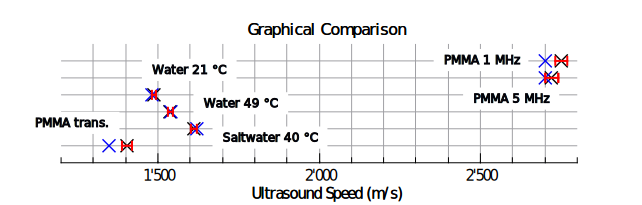
\includegraphics[scale=0.94]{results_ultrasound_speed}
	\caption{Graphical comparison between the calculated values (black cross with red uncertainty bar) and their respective literature values (blue cross). Especially the ultrasound speed of water is extremely close to the litearature value. The calculated sound velocities in PMMA at an oscillation frequency of 1 MHz are off by quite a bit (both logitudinal and transversal).}
	\label{fig:results_ultrasound_speed}
\end{figure}

\begin{figure}[H]
	\centering
	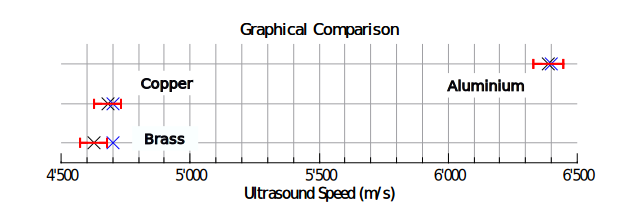
\includegraphics[scale=0.94]{results_metals}
	\caption{Graphical comparison of the three different metals aluminium, copper and brass. They are compared separately because their sound velocity is in a different range. This would have stretched out figure \ref{fig:results_ultrasound_speed} above and thus would have made it less readable. The literature values of the sound velocity (blue) in aluminium and copper lie inside the error bars of the respective metals.}
	\label{fig:results_metals}
\end{figure}

Table \ref{tab:Ultrasound_Speed} shows all calculated sound velocities and their respective literature values in one table.

\begin{table}[H]
	\centering
	\renewcommand{\arraystretch}{1.1}
	\begin{tabular}{|l|c|c|c|}
		\cline{2-4}
		\multicolumn{1}{c|}{} & $\boldsymbol{c}$ \textbf{@ 1 MHz} & $\boldsymbol{c}$ \textbf{@ 5 MHz} & \textbf{Litearture} \\
		\multicolumn{1}{c|}{} & in m/s & in m/s & in m/s \\
		\hline
		\textbf{PMMA} & $(2751\pm 19)$ & $(2721\pm 21)$ & $\approx 2700$ \\
		\hline
		\textbf{Aluminium} & - & $(6387\pm 59)$ & $\approx 6400$ \\
		\hline
		\textbf{Copper} & - & $(4680\pm 53)$ & $\approx 4700$ \\
		\hline
		\textbf{Brass} & - & $(4627\pm 52)$ & $\approx 4700$ \\
		\hline
		\textbf{Water 21 \textdegree C} & - & $(1488\pm 7)$ & $\approx 1483$ \\
		\hline
		\textbf{Water 49 \textdegree C} & - & $(1538\pm 8)$ & $\approx 1540$ \\
		\hline
		\textbf{Saltwater 40 \textdegree C} & - & $(1612\pm 10)$ & $\approx 1620$ \\
		\hline
		\textbf{PMMA trans.} & $(1405\pm 15)$ & - & $\approx 1350$ \\
		\hline
	\end{tabular}
	\caption{Summary of all calculated sound velocities and their respective literature values for the oscillation frequencies 1 MHz and 5 MHz.}
	\label{tab:Ultrasound_Speed}
\end{table}

% -----------------------------------------------------------------------------------------
\subsection{Attenuation Coefficient $\mu$}
\label{subsec:Attenuation_Coefficient}
The following figure \ref{fig:results_absorption} shows a graphical comparison between the two calculated attenuation coefficients and their uncertainties.

\begin{figure}[H]
	\centering
	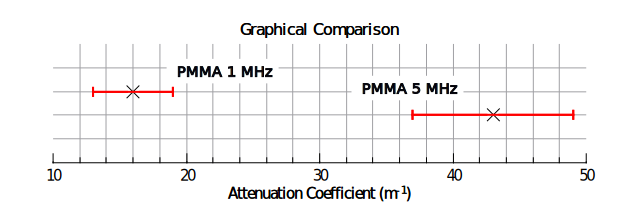
\includegraphics[scale=0.94]{results_absorption}
	\caption{Graphical comparison between the calculated values (black cross with red uncertainty bar) and their respective literature values (blue cross). The calculated attenuatin coefficient for PMMA at a frequency of 5 MHz is very imprecise. This is due to the fact, that the amplitude values are approaching 0 very fast. Thus, it is hard to get accurate readings (see figure \ref{fig:measuring_procedure}).}
	\label{fig:results_absorption}
\end{figure}

Table \ref{tab:Attenuation_Coefficient} shows the values of the calculated attenuation coefficients.

\begin{table}[H]
	\centering
	\renewcommand{\arraystretch}{1.1}
	\begin{tabular}{|l|c|c|}
		\cline{2-3}
		\multicolumn{1}{c|}{} & $\boldsymbol{\mu}$ \textbf{@ 1 MHz} & $\boldsymbol{\mu}$ \textbf{@ 5 MHz} \\
		\multicolumn{1}{c|}{} & in m$^{-1}$ & in m$^{-1}$ \\
		\hline
		\textbf{PMMA} & $(16\pm 3)$ & $(43\pm 6)$ \\
		\hline
	\end{tabular}
	\caption{Summary of the calculated attenuation coefficients for the oscillation frequencies 1 MHz and 5 MHz.}
	\label{tab:Attenuation_Coefficient}
\end{table}


% Bibliography
\printbibliography[heading=bibintoc]
\label{sec:literature}

% Glossary
\printglossaries

% Appendix
\begin{appendix}
	\section{Measurements}
	\label{sec:Measurements}
	
	\begin{table}[H]
		\centering
		\begin{tabular}{l|c|c|c|c|c}
			& \textbf{1st refl.} & \textbf{2nd refl.} & \textbf{3rd refl.} & \textbf{4th refl.} & \textbf{5th refl.} \\
			\textbf{Material} & ($\mu$s) & ($\mu$s) & ($\mu$s) & ($\mu$s) & ($\mu$s) \\
			\hline\hline
			\textbf{PMMA @ 1 MHz} & 14.878 & 29.667 & - & - & - \\ \hline
			\textbf{PMMA @ 5 MHz} & 14.903 & 29.994 & - & - & - \\ \hline
			\textbf{Aluminium} & 12.583 & 25.271 & 37.556 & - & - \\ \hline
			\textbf{Copper} & 17.224 & 34.234 & - & - & - \\ \hline
			\textbf{Brass} & 18.041 & 34.870 & 52.109 & - & - \\ \hline
			\textbf{Water 21 \textdegree C} & 25.200 & 65.754 & 133.440 & 186.695 & 240.265 \\ \hline
			\textbf{Water 49 \textdegree C} & 24.148 & 64.144 & 129.150 & 180.400 & 232.590 \\ \hline
			\textbf{Saltater 40 \textdegree C} & 22.682 & 60.532 & 123.192 & 172.070 & 221.240 \\ \hline
			\textbf{PMMA trans. @ 1 MHz} & 28.533 & 58.087 & - & - & - \\ \hline
		\end{tabular}
		\caption{This table shows the measured time of flights. The metals and the liquids were measured at a frequency of 5 MHz.}
		\label{tab:Slit_Measurements}
	\end{table}

	\begin{table}[H]
		\centering
		\begin{tabular}{l|c|c|c}
			& \textbf{1st ampl.} & \textbf{2nd ampl.} & \textbf{3rd ampl.} \\
			\textbf{Material} & (V) & (V) & (V) \\
			\hline\hline
			\textbf{PMMA @ 1 MHz} & 2.02 & 1.09 & 0.50 \\ \hline
			\textbf{PMMA @ 5 MHz} & 2.39 & 0.43 & 0.01 \\ \hline
		\end{tabular}
		\caption{This table shows the measured amplitudes in PMMA at 1 MHz and 5 MHz.}
		\label{tab:Slit_Measurements}
	\end{table}

	\newpage

	\section{MATLAB Error Calculation}
	\label{sec:MATLAB_Error_Calculation}
	\lstinputlisting{appendix/Error_Calculation.m}
\end{appendix}


% Debug
\ifdraft{
	\newpage
	\listoftodos[\section{To-Do}]
	\clearpage
}
{
}

\end{document}
